%
% $RCSfile: software_engineering_process.tex,v $
%
% Copyright (c) 2002-2007. Christian Heller. All rights reserved.
%
% Permission is granted to copy, distribute and/or modify this document
% under the terms of the GNU Free Documentation License, Version 1.1 or
% any later version published by the Free Software Foundation; with no
% Invariant Sections, with no Front-Cover Texts and with no Back-Cover
% Texts. A copy of the license is included in the section entitled
% "GNU Free Documentation License".
%
% http://www.cybop.net
% - Cybernetics Oriented Programming -
%
% Version: $Revision: 1.1 $ $Date: 2007-07-17 20:02:36 $ $Author: christian $
% Authors: Christian Heller <christian.heller@tuxtax.de>
%

\subsection{Software Engineering Process}
\label{software_engineering_process_heading}
\index{Software Engineering Process}

Although hundreds of variations, with or without iterations, exist, a standard
\emph{Software Engineering Process} (SEP) consists of the phases: \emph{Analysis},
\emph{Design} and \emph{Implementation}, as illustrated in figure
\ref{software_engineering_process_figure}.

\begin{figure}[ht]
    \begin{center}
        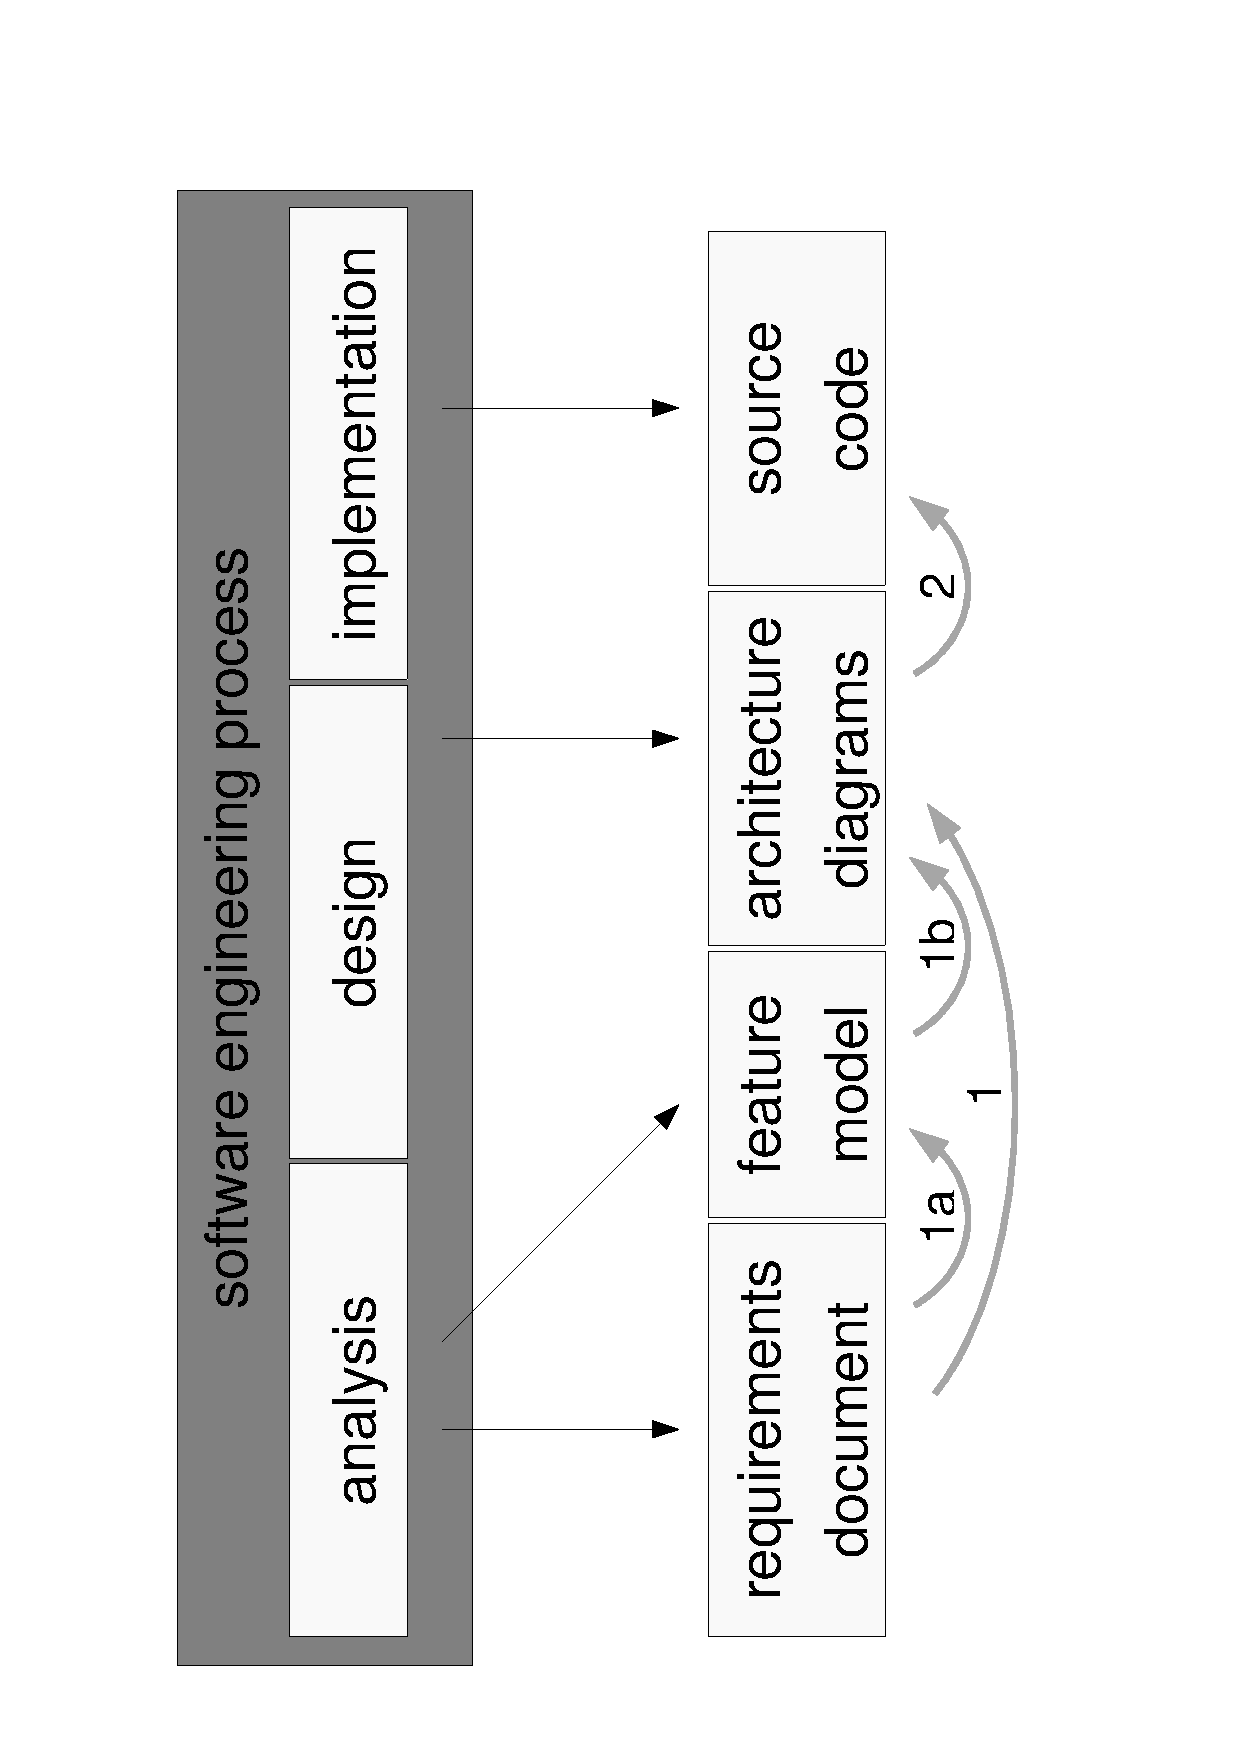
\includegraphics[scale=0.3,angle=-90]{graphics/gaps.pdf}
        \caption{Standard Software Engineering Process}
        \label{software_engineering_process_figure}
    \end{center}
\end{figure}
